% Created 2020-04-29 Wed 18:43
% Intended LaTeX compiler: pdflatex
\documentclass[12pt]{report}
\usepackage[utf8]{inputenc}
\usepackage[T1]{fontenc}
\usepackage{graphicx}
\usepackage{grffile}
\usepackage{longtable}
\usepackage{wrapfig}
\usepackage{rotating}
\usepackage[normalem]{ulem}
\usepackage{amsmath}
\usepackage{textcomp}
\usepackage{amssymb}
\usepackage{capt-of}
\usepackage{hyperref}
\setlength{\parindent}{0pt}
\usepackage[margin=1.6in]{geometry}
\usepackage{emptypage}
\usepackage{tikz}
\usetikzlibrary{graphs,graphs.standard,bayesnet,arrows.meta,shapes.arrows}

% Colorlinks sets pdfborder to zero.
%\hypersetup{colorlinks,linkcolor=,urlcolor=gray}

%\usepackage[a4paper,top=2.25cm,bottom=2.25cm,left=3.0cm,right=3.0cm]{geometry}

%% arial font?????????
%% \usepackage[scaled]{uarial}
%% \renewcommand*\familydefault{\sfdefault} %% Only if the base font of the document is to be sans serif
%% \usepackage[T1]{fontenc}

\makeatletter
\renewenvironment{abstract}{%
    \if@twocolumn
      \section*{\abstractname}%
    \else %% <- here I've removed \small
      \begin{center}%
        {\bfseries \Huge\abstractname\vspace{\z@}}%  %% <- here I've added \Large
      \end{center}%
      \quotation
    \fi}
    {\if@twocolumn\else\endquotation\fi}
\makeatother

%\pagecolor{yellow!10}

\documentclass{book}
\usepackage{sectsty}
\chapternumberfont{\large} 
\chaptertitlefont{\huge}

\usepackage{hyperref}
\hypersetup{%
  colorlinks=false,% hyperlinks will be black
  linkbordercolor=red,% hyperlink borders will be red
  pdfborderstyle={/S/U/W 1}% border style will be underline of width 1pt
}

%% \usepackage[T1]{fontenc}
%% \usepackage{libertine}
%% \usepackage{graphicx}
%% \usepackage[svgnames]{xcolor}
%% \usepackage{framed}

%% \newcommand*\openquote{\makebox(25,-22){\scalebox{5}{``}}}
%% \newcommand*\closequote{\makebox(25,-22){\scalebox{5}{''}}}
%% \colorlet{shadecolor}{Azure}

%% \makeatletter
%% \newif\if@right
%% \def\shadequote{\@righttrue\shadequote@i}
%% \def\shadequote@i{\begin{snugshade}\begin{quote}\openquote}
%% \def\endshadequote{%
%%   \if@right\hfill\fi\closequote\end{quote}\end{snugshade}}
%% \@namedef{shadequote*}{\@rightfalse\shadequote@i}
%% \@namedef{endshadequote*}{\endshadequote}
%% \makeatother
%% \begin{document}


\author{Louis James}
\date{\today}
\title{Spatial memory, embodied thinking, computer vision projection application \\
or \\
Exploring cognition and interaction in a spatial and physicalised computer environment. \\
or \\
A system for exploring haptic and spatial interaction environments}
\hypersetup{
 pdfauthor={Louis James},
 pdftitle={Spatial memory, embodied thinking, computer vision projection application \\
or \\
Exploring cognition and interaction in a spatial and physicalised computer environment. \\
or \\
A system for exploring haptic and spatial interaction environments},
 pdfkeywords={},
 pdfsubject={Final year project for Creative Computing},
 pdfcreator={Emacs 26.3 (Org mode 9.3.6)}, 
 pdflang={English}}
\begin{document}

\maketitle

\renewcommand{\abstractname}{Acknowledgements}
\begin{abstract}
 Thanks to my family, Florent, Chudleigh dwellers, Jamie ...
\end{abstract}
\newpage

\renewcommand{\abstractname}{Abstract}
\begin{abstract}
This project\ldots{}
\end{abstract}
\tableofcontents
\chapter{Introduction}
\label{sec:orgfdd50b0}
\chapter{Background}
\label{sec:org43f6876}

The motivation for this project stems in part from a feeling of frustration in
how working on computers can often be a constricted affair and a pondering over
how we might expand the \emph{keyboard-mouse-monitor} model to improve the utility of
computers regarding our own perceptive abilities. How might a spatial and more
\emph{haptic} environment for interaction create an improved space for thinking with
computers as well as our physical health.

\section{Definitions}
\label{sec:org917710e}
\begin{enumerate}
\item Computing
\label{sec:org32fe2f3}
\item keyboard-mouse-monitor model (kmm model) (?)
\label{sec:orgc511e0d}
\end{enumerate}

\section{Original ideas with exocortexes; Externalised memory and organisational systems}
\label{sec:org36a782a}

\begin{enumerate}
\item Org mode and nataniev ecosystem
\label{sec:org7fdf1b4}
\end{enumerate}

\section{Dynamicland}
\label{sec:org977886d}

One of my original points of reference was \emph{Dynamicland}, a research project in
Oakland, USA. The aim of the project is to implement a new more powerful and
accessible model of computing.

\begin{quote}


In Oakland, we built the first full-scale realization of the vision, inviting
thousands of people into our space to collaborate. Together, these artists,
scientists, teachers, students, programmers, and non-programmers created
hundreds of projects that would have been impossible anywhere else.
-- Dynamicland.org
\end{quote}

\emph{Dynamicland} is a communal computer where the building is the computer (a
transition back in scale to the days of the first computers ENIAC). Programs are
embodied in the room on pieces of colour-coded paper. The programs are
recognised via the codes and their code, stored in a database is then run. It
can also \emph{read} code using OCR but generally the code is there \href{https://thenewstack.io/dynamicland-rethinks-computer-interfaces/}{symbolically}. 

\begin{figure}[htbp]
\centering
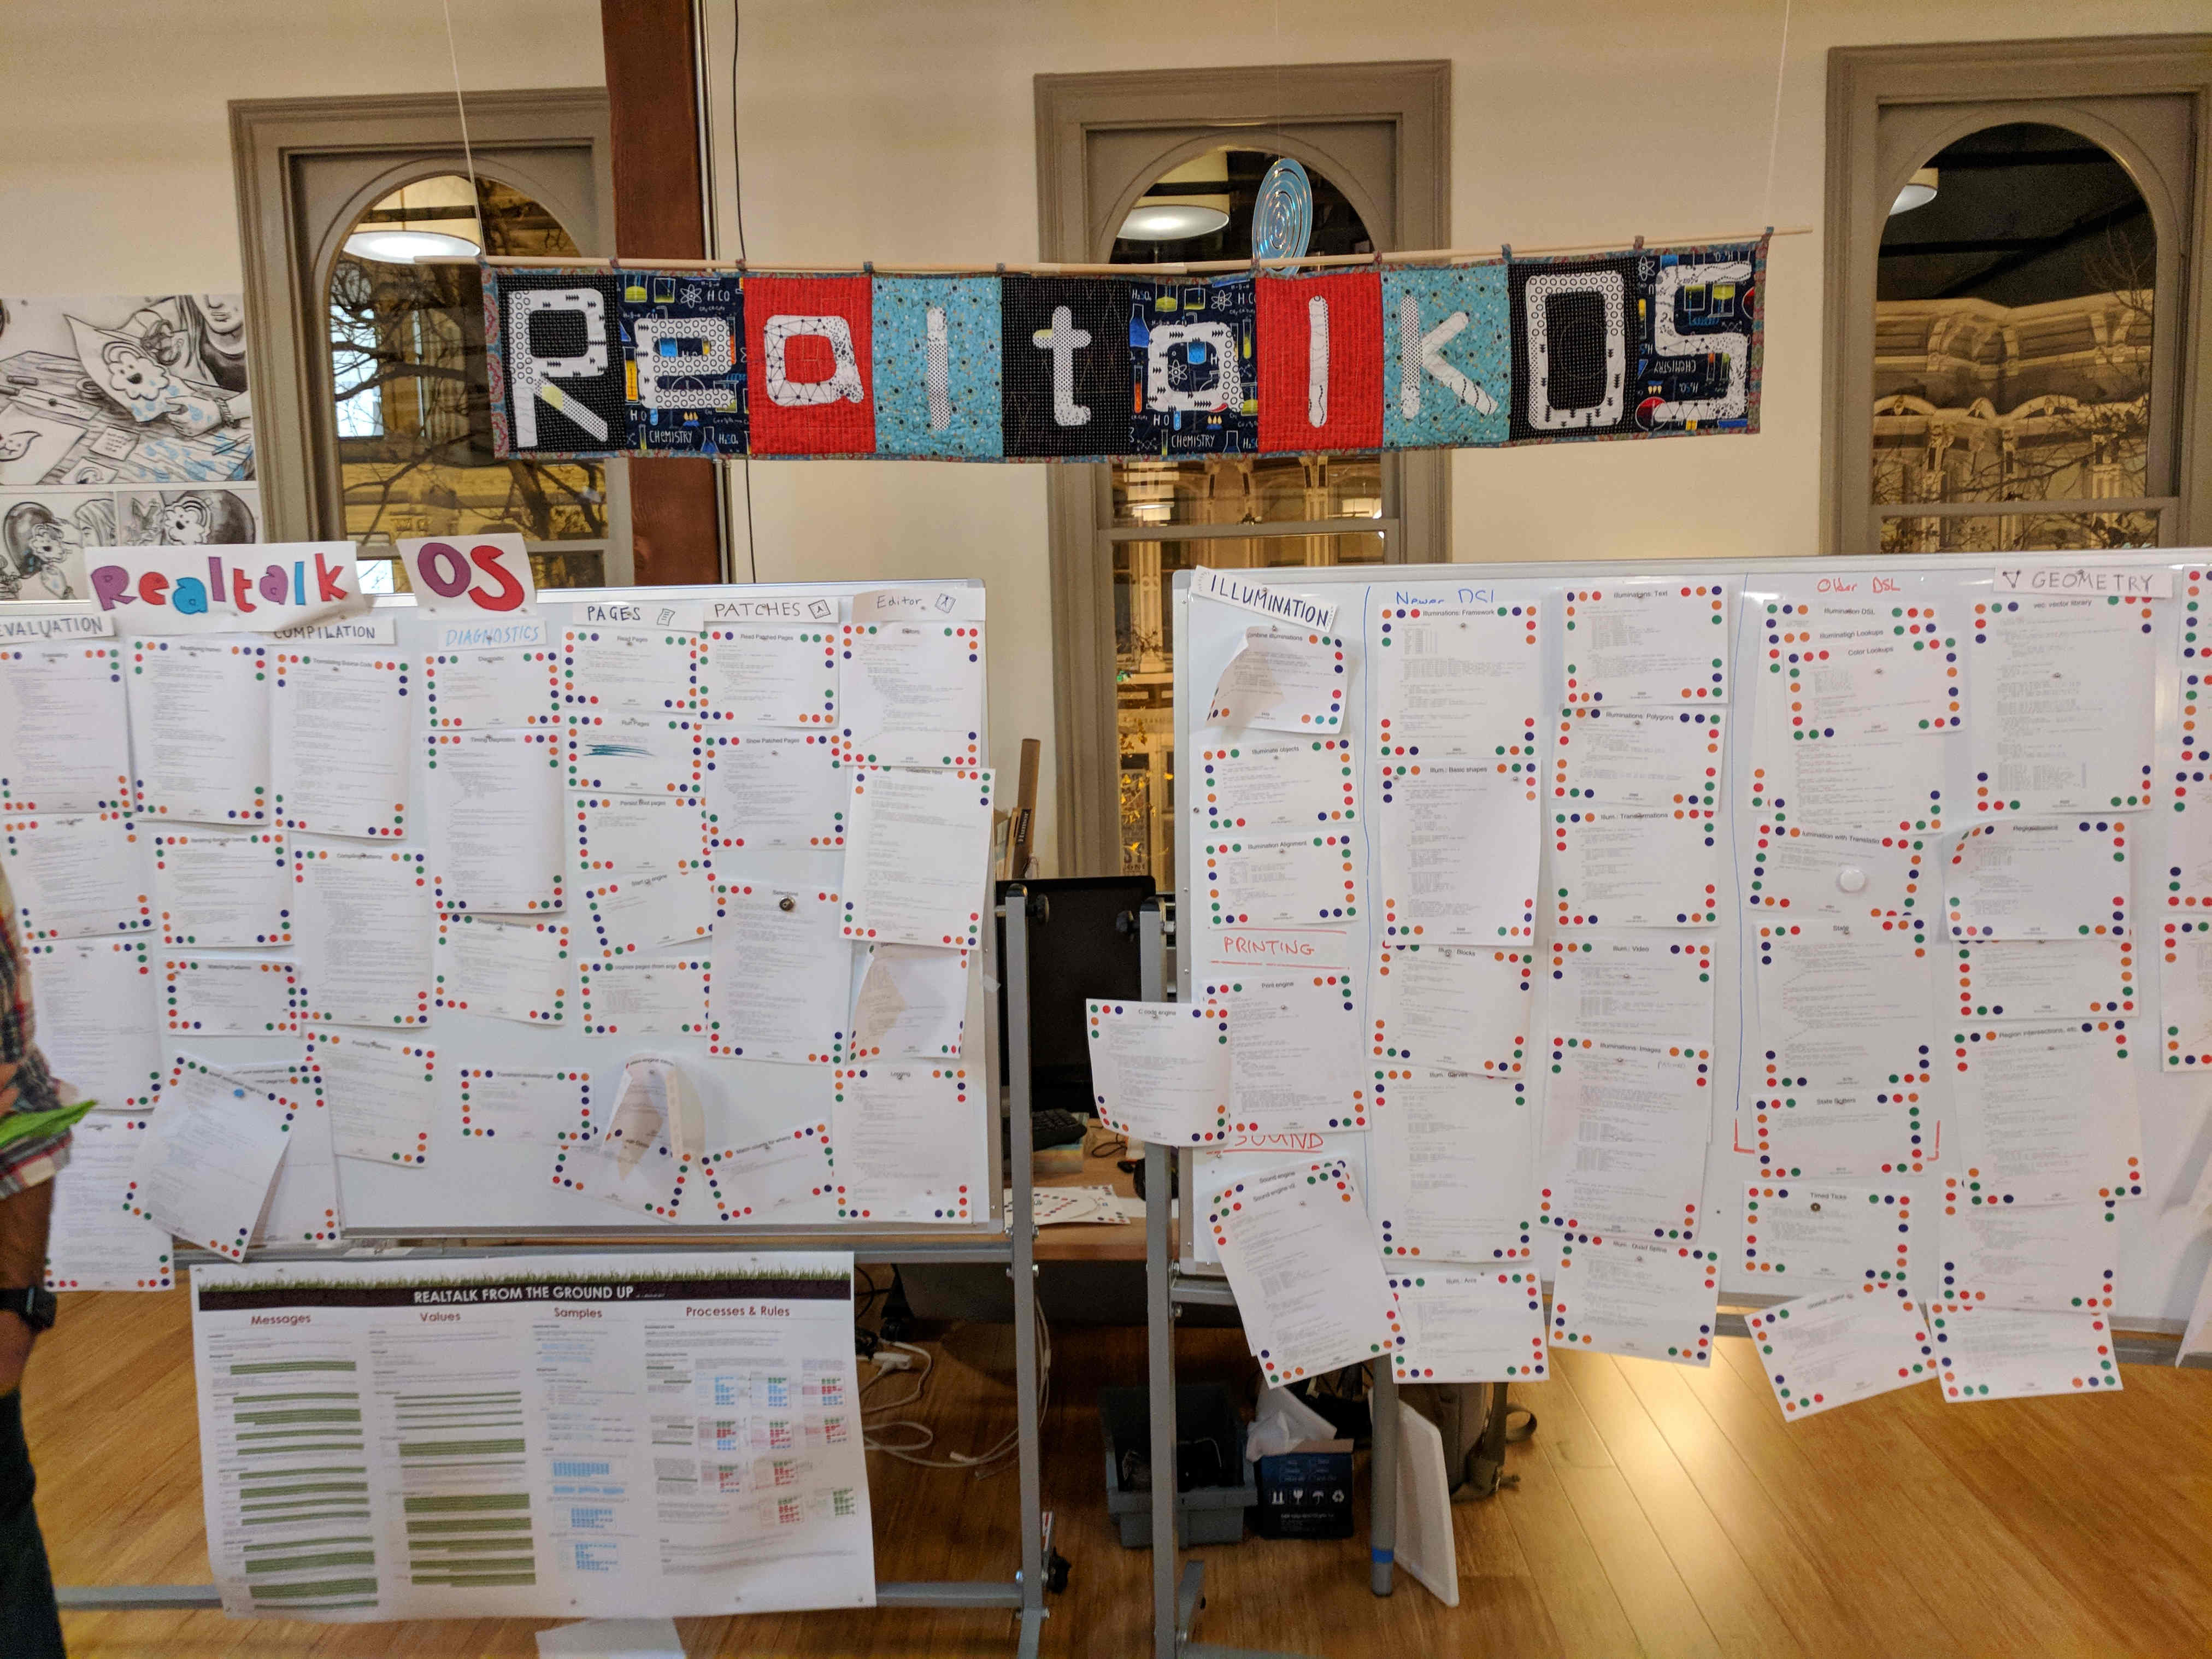
\includegraphics[width=.9\linewidth]{assets/realtalk-os.jpg}
\caption{RealtalkOS, the operating system of Dynamicland}
\end{figure}

\begin{enumerate}
\item Dynamiclands opensource model
\label{sec:orga1b94f2}
\end{enumerate}


\section{Paper programs - open source}
\label{sec:orge34c9bc}

\section{Sage digital research}
\label{sec:org4488537}

\section{Design of everyday things?}
\label{sec:orge176ef2}

\section{Nielsen: augmenting ltm and using ai to augment human-i}
\label{sec:org1dea1c8}

\section{mental and physical health implications of contemporary computing ? Are they really quite minor?}
\label{sec:orgefe4cfe}

\section{Computational creativity?}
\label{sec:org360622a}

\begin{enumerate}
\item Open source
\label{sec:org2d1dae3}

\item alex mclean thesis
\label{sec:org8010e45}

\item 
\label{sec:org0ae3e29}
\end{enumerate}

\chapter{Specification and context}
\label{sec:orgedefed5}
\chapter{Project in depth}
\label{sec:org3dc1183}
\chapter{Creative process}
\label{sec:org69b5cef}
\chapter{Debugging and problem solving}
\label{sec:orge8abb54}
\chapter{Evaluation and Conclusions}
\label{sec:org4ba246a}
\bibliographystyle{ieeetr} 
\bibliography{references}

\chapter{Appendix}
\label{sec:orgb07a881}
\end{document}
